\documentclass[11pt,a4paper]{article}
\usepackage[czech]{babel}
\usepackage[utf8]{inputenc}
\usepackage[IL2]{fontenc}
\usepackage[top=3cm, left=2cm, text={17cm, 24cm}]{geometry}
\usepackage{times}
\usepackage{multirow}
\usepackage{graphicx}
\usepackage[ruled,czech]{algorithm2e}
\usepackage{algorithmic}

\renewcommand{\algorithmicrequire}{\textbf{Input:}}
\renewcommand{\algorithmicensure}{\textbf{Output:}}
\renewcommand{\algorithmicto}{to}
\algsetup{indent=2em}

\begin{document}

\begin{titlepage}
  \begin{center}
    \Huge \textsc{Vysoké učení technické v~Brně \\
    \huge Fakulta informačních technologií\\
    \vspace{\stretch{0.382}}}
    \LARGE Typografie a~publikování\,--\,3. projekt\\
    \Huge Tabulky a~obrázky\\
    \vspace{\stretch{0.618}}
  \end{center}
  \Large \today \hfill Pavel Frýz
\end{titlepage}

\section{Úvodní strana}
  Název práce umístěte do zlatého řezu a~nezapomeňte uvést dnešní datum a~vaše jméno
  a~příjmení.

\section{Tabulky}
  Pro sázení tabulek můžeme použít buď prostředí\texttt{ tabbing }nebo prostředí\texttt{
  tabular}.

\subsection{Prostředí\texttt{ tabbing}}
  Při použití\texttt{ tabbing }vypadá tabulka následovně:
  \begin{tabbing}
    Vodní melouny \quad \= 25,90 \quad \=                \kill
    \textbf{Ovoce} \> \textbf{Cena} \> \textbf{Množství} \\
    Jablka         \> 25,90         \> 5\,kg             \\
    Hrušky         \> 27,40         \> 2,5\,kg           \\
    Vodní melouny  \> 35,--         \> 1\,kus            \\
  \end{tabbing}
  Toto prostředí se dá také použít pro sázení algoritmů, ovšem vhodnější je použít
  prostředí\texttt{ algorithm }nebo\texttt{ algorithm2e }(viz sekce \ref{algo}).

\subsection{Prostředí\texttt{ tabular}}
  Další možností, jak vytvořit tabulku, je použít prostředí\texttt{ tabular}. Tabulky pak
  budou vypadat takto\footnote{Kdyby byl problem s\texttt{~cline, }zkuste se podívat třeba
  sem: http://www.abclinuxu.cz/tex/poradna/show/325037}:

  \begin{table}[ht]
    \catcode`\-=12
    \begin{center}
      \begin{tabular}{|l|r|r|}                               \hline
                      & \multicolumn{2}{c|}{\textbf{Cena}} \\\cline{2-3}
        \textbf{Měna} & \textbf{nákup} & \textbf{prodej}   \\\hline
        EUR           & 24,501         & 24,324            \\
        JPY           & 105,484        & 105,847           \\
        USD           & 16,632         & 16,328            \\\hline
      \end{tabular}
      \caption{Tabulka kurzů k dnešnímu dni}
      \label{tab1}
    \end{center}
  \end{table}

  \begin{table}[ht]
    \catcode`\-=12
    \begin{center}
      \begin{tabular}{|c|c|}    \hline
        $A$        & $\neg A$ \\\hline
        \textbf{P} & N        \\\hline
        \textbf{X} & X        \\\hline
        \textbf{N} & P        \\\hline
      \end{tabular}
      \begin{tabular}{|c|c|c|c|c|}\hline
        \multicolumn{2}{|c}{} & \multicolumn{3}{|c|}{$B$}\\\cline{3-5}
        \multicolumn{2}{|c|}{$A \wedge B$} & \textbf{P} & \textbf{X} & \textbf{N} \\\hline
        \multirow{3}{*}{$A$}
          & \textbf{P} & P & X & N \\\cline{2-5}
          & \textbf{X} & X & X & N \\\cline{2-5}
          & \textbf{N} & N & N & N \\\hline
      \end{tabular}
      \begin{tabular}{|c|c|c|c|c|}\hline
        \multicolumn{2}{|c}{} & \multicolumn{3}{|c|}{$B$}\\\cline{3-5}
        \multicolumn{2}{|c|}{$A \vee B$} & \textbf{P} & \textbf{X} & \textbf{N} \\\hline
        \multirow{3}{*}{$A$}
          & \textbf{P} & P & P & P \\\cline{2-5}
          & \textbf{X} & P & X & X \\\cline{2-5}
          & \textbf{N} & P & X & N \\\hline
      \end{tabular}
      \begin{tabular}{|c|c|c|c|c|}\hline
        \multicolumn{2}{|c}{} & \multicolumn{3}{|c|}{$B$}\\\cline{3-5}
        \multicolumn{2}{|c|}{$A \rightarrow B$} & \textbf{P} & \textbf{X} & \textbf{N} \\\hline
        \multirow{3}{*}{$A$}
          & \textbf{P} & P & X & N \\\cline{2-5}
          & \textbf{X} & P & X & P \\\cline{2-5}
          & \textbf{N} & P & P & P \\\hline
      \end{tabular}
      \caption{Kleeneho trojhodnotová logika}
      \label{tab2}
    \end{center}
  \end{table}

\section{Algoritmy} \label{algo}
  Pokud budeme chtít vysázet algoritmus, můžeme použít prostředí\texttt{ algorithm}\footnote{
  Pro nápovědu, jak zacházet s~prostředím\texttt{ algorithm, }můžeme zkusit
  tuhle stránku: \\http://ftp.cstug.cz/pub/tex/CTAN/macros/latex/contrib/algorithms/algorithms.pdf.}
  nebo\texttt{ algorithm2e}\footnote{Pro\texttt{ algorithm2e }zase tuhle:
  http://ftp.cstug.cz/pub/tex/CTAN/macros/latex/contrib/algorithm2e/algorithm2e.pdf.}.\texttt{ }
  Příklad použití prostředí\texttt{ algorithm2e }viz Algoritmus \ref{alg1}.
  \begin{algorithm}
    \caption{\sc FastSLAM}
    \label{alg1}
    \begin{algorithmic}[1]
      \REQUIRE $(X_{t-1},u_t,z_t)$
      \ENSURE $X_t$
      \medskip
      \STATE $\overline{X_t}=X_t=0$
      \FOR{$k=1$ \TO $M$}
        \STATE $x_t^{[k]}=\emph{sample\_motion\_model}(u_t,x_{t-1}^{[k]})$
        \STATE $\omega_t^{[k]}=\emph{measurement\_model}(z_t,x_t^{[k]},m_{t-1})$
        \STATE $m_t^{[k]}=updated\_occupancy\_grid(z_t,x_t^{[k]},m_{t-1}^{[k]})$
        \STATE $\overline{X_t}=\overline{X_t}+\langle x_x^{[m]},\omega_t^{[m]}\rangle$
      \ENDFOR
      \FOR{$k=1$ \TO $M$}
        \STATE draw $i$ with probability $\approx \omega_t^{[i]}$
        \STATE add $\langle x_x^{[k]},m_t^{[k]}\rangle$ \TO $X_t$
      \ENDFOR
      \RETURN{$X_t$}
    \end{algorithmic}
  \end{algorithm}

\section{Obrázky}
  Do našich článků můžeme samozřejmě vkládat obrázky. Pokud je obrázkem fotografie,
  můžeme klidně použít bitmapový soubor. Pokud by to ale mělo být nějaké schéma nebo
  něco podobného, je dobrým zvykem takovýto obrázek vytvořit vektorově.
  \begin{figure}[ht]
    \centering
    \scalebox{0.4}{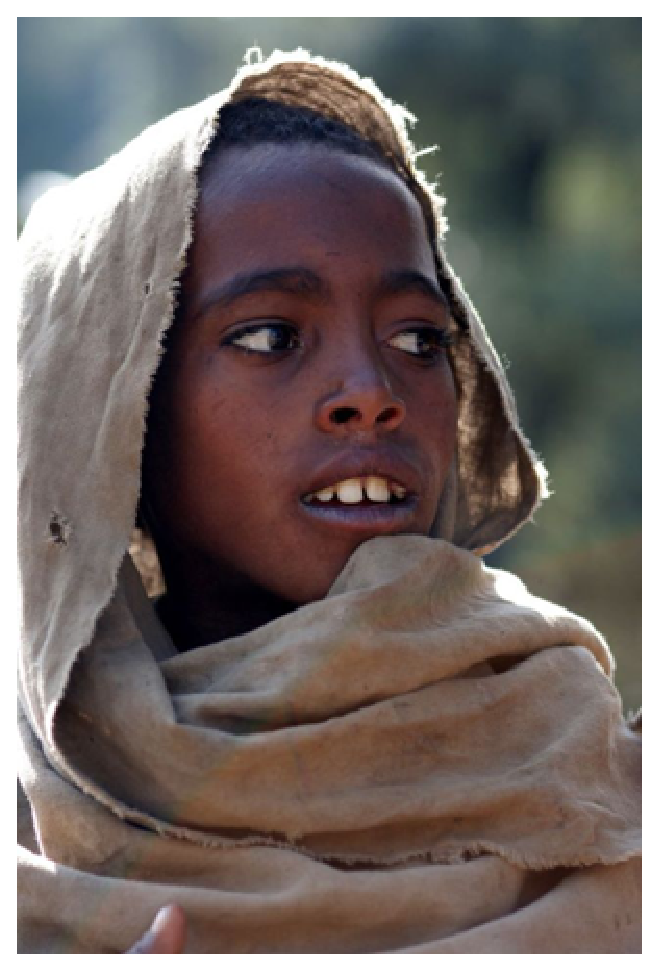
\includegraphics{etiopan.eps}
    \reflectbox{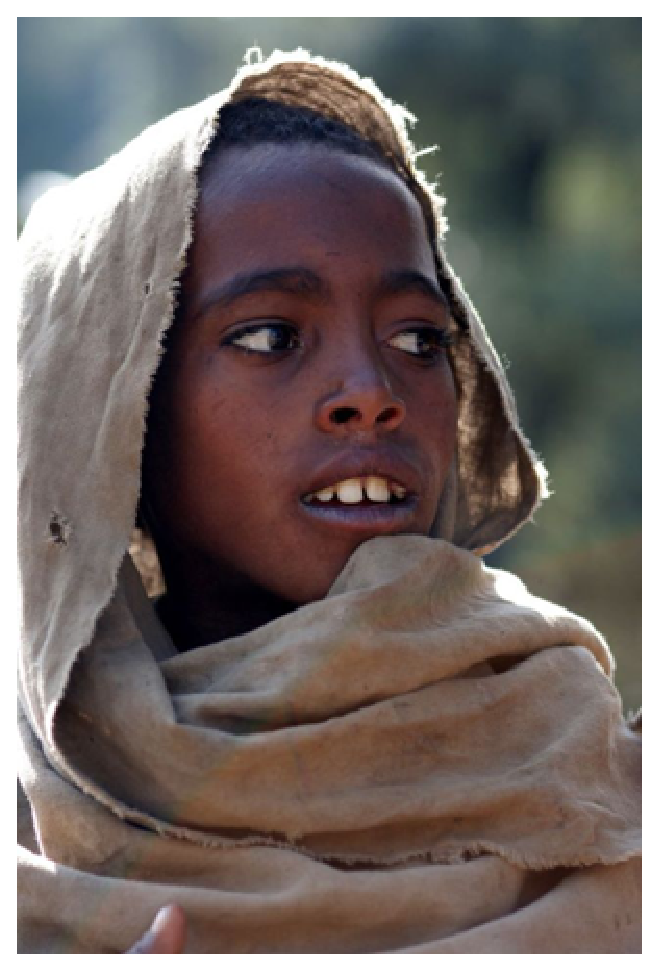
\includegraphics{etiopan.eps}} }
    \caption{Malý etiopánek a jeho bratříček}
    \label{ob1}
  \end{figure}
  \newpage
  Rozdíl mezi vektorovým\,\dots
  \begin{figure}[ht]
    \centering
    \scalebox{0.4}{
\includegraphics{oniisan.eps}}
    \caption{Vektorový obrázek}
    \label{ob2}
  \end{figure}

  \noindent
  \dots\,a bitmapovým obrázkem
  \begin{figure}[ht]
    \centering
    \scalebox{0.6}{
\includegraphics{oniisan2.eps}}
    \caption{Bitmapový obrázek}
    \label{ob3}
  \end{figure}

  \noindent
  se projeví například při zcětšení.

  Odkazy (nejen ty) na obrázky \ref{ob1}, \ref{ob2} a~\ref{ob3}, na tabulky \ref{tab1}
  a~\ref{tab2} a~také na algoritmus \ref{alg1} jsou udělány pomocí křížových odkazů. Pak je ovšem
  potřeba zdrojový soubor přeložit dvakrát.

  Vektorové obrázky lze vytvořit i~přímo v~\LaTeX u, například pomocí prostředí
  \texttt{picture}. Všechny rozměry jsou uváděny v~mm.

  \begin{figure}[p]
    \centering
    \setlength{\unitlength}{1.35mm}
    \begin{picture}(115,158.5)
      \put(0,0){\thicklines\framebox(115,158.5)}
      \multiput(15,158.5)(0,-10){16}{\line(0,-1){7}}
      \multiput(0,144)(10,0){11}{\line(1,0){7}}
      \put(0,3){\vector(-1,0){0}\vector(1,0){115}}
      \put(0,4){\makebox(115,10)[b]{Šířka stránky = 115}}
      \put(112,0){\vector(0,-1){0}\vector(0,1){158.5}}
      \put(102,57){\vector(1,1){10}}
      \put(92,52){\makebox(20,0){\shortstack{Výška\\stránky = 158.5}}}
      \put(88,158.5){\vector(0,1){0}\vector(0,-1){14.5}}
      \put(88,152){\makebox(20,0){\shortstack{Výška\\mezery = 14,5}}}
      \put(88,144){\vector(0,1){0}\vector(0,-1){10}}
      \put(88,139){\makebox(19,0){\shortstack{Výška\\mezery = 10}}}
      \put(88,134){\vector(0,1){0}\vector(0,-1){10}}
      \put(88,129){\makebox(20,0){\shortstack{Výška\\hlavičky = 10}}}
      \put(88,124){\vector(0,1){0}\vector(0,-1){14}}
      \put(88,117){\makebox(19,0){\shortstack{Výška\\mezery = 14}}}
      \put(88,110){\vector(0,1){0}\vector(0,-1){75}}
      \put(88,65){\makebox(15,0){\shortstack{Výška\\těla = 75}}}
      \put(88,35){\vector(0,1){0}\vector(0,-1){15}}
      \put(88,27){\makebox(19,0){\shortstack{Výška\\mezery = 15}}}
      \put(88,20){\vector(0,1){0}\vector(0,-1){10}}
      \put(88,14){\makebox(16,0){\shortstack{Výška\\paty = 10}}}
      \put(0,93){\vector(-1,0){0}\vector(1,0){15}}
      \put(0,94){\makebox(15,10)[b]{Mezera = 15}}
      \put(85,93){\vector(-1,0){0}\vector(1,0){9}}
      \put(94,105){\vector(-1,-3){4}}
      \put(92,107){\makebox(10,0){Mezera = 9}}
      \put(94,93){\vector(-1,0){0}\vector(1,0){15}}
      \put(94,94){\makebox(15,10)[b]{\shortstack{Šířka\\boxu = 15}}}
      \put(30,137){\vector(-1,0){0}\vector(1,0){55}}
      \put(30,138){\makebox(55,10)[b]{Šířka boxu = 55}}
      \put(30,124){\thicklines\framebox(55,10){\bf Hlavička}}
      \put(30,35){\thicklines\framebox(55,75){\bf Textové tělo}}
      \put(30,10){\thicklines\framebox(55,10){\bf Pata}}
      \put(94,79.5){\thicklines\framebox(15,10){\shortstack{\bf Okrajová\\\bf poznámka}}}
    \end{picture}
  \caption{Vektorový obrázek v prostředí \texttt{picture}.}
  \end{figure}

\end{document}